%%%%%%%%%%%%%%%%%%%%%%%%%%%%%%%%%%%%%%%%%%%%%%%%%%%%%%%%%
%%%%%IMPORTS:
%packages a utilizar:
\documentclass{report}
\usepackage[T1]{fontenc}     % Fontes T1
\usepackage[utf8]{inputenc}  % Input UTF8
\usepackage[top=3cm,bottom=3cm,left=3cm,right=2.5cm,asymmetric]{geometry} %fronteiras
%\usepackage[nottoc]{tocbibind}
\usepackage[table]{xcolor} %Colorir tabelas
\usepackage[backend=biber, style=ieee]{biblatex} %bibliografia
\usepackage{csquotes}  % referências
\usepackage[portuguese]{babel} %Usar língua portuguesa
\usepackage{blindtext} 
\usepackage[printonlyused]{acronym}  %Acrónimos
\usepackage{hyperref}  %Autoref no índice
\usepackage{graphicx}  %Usar imagens
\usepackage{titling}
\usepackage{multicol} %multicoluna de texto
\usepackage{adjustbox}
\renewcommand{\figurename}{Fig.} 
\renewcommand{\tablename}{Tabela} 
\usepackage[font=small,tableposition=top]{caption} 
\usepackage[font=small]{subcaption}
\usepackage{xcolor} %cor nos textos
\usepackage{amsmath} %matematica
\usepackage{amssymb} %simbolos matematicos
\graphicspath{ {./images/} } %directorio das imagens
\usepackage{fancyhdr}
\usepackage{authblk}
\usepackage{float} %Posicionamento exacto das figuras no texto
\usepackage{url}   %referencias URL
\usepackage{blindtext}
\def\UrlBreaks{\do\/\do-} %não cortar referencias

\usepackage{indentfirst} %Garantir avanço do primeiro parágrafo
\hypersetup{pdfborder=0 0 0} %Remover a caixa vermelha das referências
\usepackage{chngcntr} %Numeração contínua das figuras
\counterwithout{figure}{chapter} %Numeração contínua de figuras
\counterwithout{table}{chapter} %Numeração contínnua de tabelas
\setlength{\parskip}{0.2cm} %Aumento de espaçamento entre parágrafos

\usepackage{hyperref}


\begin{document}	
	%Definições do Relatório

%Dados Gerais:
\def\titulo{Projecto Final: \\ Máquina de Lavagem de Roupa}
\def\data{Junho de 2022}
\def\versao{Ver.: 1.13}
\def\departamento{Departamento de Electrónica Telecomunicações e Informática}
\def\empresa{Universidade de Aveiro}
\def\logotipo{logotipo_ua.png}

%Dados dos Autores:
%primeiro autor:
\def\pautor{João Pedro Nunes Vieira} 
\def\numpautor{Nº Mec.:  50458}
\def\contactopautor{joaopvieira@ua.pt}
%segundo autor:
\def\sautor{Leandro Roque Costa} 
\def\numsautor{Nº Mec.: 110326}
\def\contactosautor{lrc@ua.pt}
%
\def\autores{\pautor \\ \sautor}

	%Capa do Relatório:
\begin{titlepage} 
	\begin{center}
	\includegraphics[scale=0.50]{\logotipo}
	\line(1,0){350} \\ 
		\vspace*{2mm}
	{\Large \uc} \\
		\vspace*{2mm} 	
	{\Huge \titulo} \\
		\vspace*{2mm}
	\line(1,0){350} \\ 
		\vspace*{2mm}
	{\Large \empresa} \\
		\vspace*{20mm}
	{\Large \autores} \\ 
		\vspace*{\fill}
	\end{center}

	\begin{flushright} 
		{\large \departamento} \\ 
		{\versao} 
	\end{flushright}

\end{titlepage}

	%Página de Título:
\predate{\begin{flushright}\small}
\postdate{\par\end{flushright}}

\title{ 
	{\huge\textbf{\titulo} } \\ 
	{\large \departamento\\ \empresa} }

\author{

    \begin{tabular}{l}
        \pautor, \numpautor\hfil \\
        \contactopautor
    \end{tabular}
    \and
    \begin{tabular}{l}
        \sautor, \numsautor\hfil \\
        \contactosautor
    \end{tabular}
    \and
    \begin{tabular}{l}
        \tautor, \numtautor\hfil \\
        \contactotautor
    \end{tabular}
    \and
    \begin{tabular}{l}
        \qautor, \numqautor\hfil \\
        \contactoqautor
    \end{tabular}
}




\date{\vspace{\fill}{\data}} 
\maketitle
	\begin{abstract}

O presente relatório aborda a comunicação entre aplicações seguindo um modelo Cliente-Servidor, usando conceitos abordados no decorrer da Unidade Curricular de Laboratórios de Informática, nomeadamente programação de sockets TCP, Criptografia, Documentação JSON, programação em Python, etc... \\
Este trabalho é relevante pois com o avanço tecnológico actual, a aprendizagem dos conceitos anteriormente referidos torna-se imperativa para os estudantes de cursos ligados à tecnologia de informação.\\
O projecto foi realizado por duas pessoas, tendo como objectivo o desenvolvimento das capacidades de trabalho em grupo, desenvolvimento e estruturação de código, realização de testes funcionais e planeamento através da plataforma \textbf{code.ua.pt}. \\
Foi possível implementar com sucesso um modelo de comunicação entre aplicações Cliente-Servidor em gênero "Jogo High-Low" com funcionalidade de segurança(encriptação) de forma simples, prática e eficaz, conseguindo-se corrigir todos os erros encontrados.

\end{abstract}
	
%%%%%%%%%%%%%%%%%%%%%%%%%%%%%%%%%%%%%%%%%%%%%%%%%%%%%%%%%
%%%%%INDICE:

\renewcommand{\contentsname}{Índice}
\tableofcontents
\listoffigures
\pagenumbering{roman}

%%%%%%%%%%%%%%%%%%%%%%%%%%%%%%%%%%%%%%%%%%%%%%%%%%%%%%%%%
%%%%%ACRÓNIMOS:

\chapter*{Acrónimos}
\begin{acronym}

\acro{ua}[UA]{Universidade de Aveiro}
\acro{deti}[DETI]{Departamento de Eletrónica, Telecomunicações e Informática}
\acro{leci}[LECI]{Licenciatura em Engenharia de Computadores e Informática}
\acro{uc}[UC]{Unidade Curricular}
\acro{sio}[SIO]{Segurança Informática e Nas Organizações} 
\acro{cwe}[CWE]{Common Weakness Enumeration}
\acro{asvs}[ASVS]{Application Security Verification Standard}
\acro{www}[WWW]{World Wide Web}
\acro{sio}[SIO]{Segurança Informática e nas Organizações}
\acro{mfa}[MFA]{Multi-factor Authentication}
\acro{jwt}[JWT]{JSON Web Token}
\acro{oidc}[OIDC]{OpenID Connect}
\end{acronym}

%%%%%%%%%%%%%%%%%%%%%%%%%%%%%%%%%%%%%%%%%%%%%%%%%%%%%%%%%
%%%%%HEADERS & FOOTERS:

\pagestyle{fancy}
\fancyhf{}
\chead{\titulo}
\cfoot{\thepage}
%%%%%%%%%%%%%%%%%%%%%%%%%%%%%%%%%%%%%%%%%%%%%%%%%%%%%%%%%
%%%%%%%%%%%%%%%%%%%%%%%%%%%%%%%%%%%%%%%%%%%%%%%%%%%%%%%%%
%%%%%INTRODUÇÃO:
%
\chapter{Introdução}
\label{chap.Intro}
\pagenumbering{arabic}

O \ac{asvs} representa um guia essencial de requisitos e testes de segurança para aplicações, destacando-se como uma ferramenta crucial para profissionais que se dedicam ao desenvolvimento de soluções informáticas seguras. Este projeto tem como objetivo principal aperfeiçoar e melhorar a loja online original do \ac{deti} por forma a cumprir os requisitos estabelecidos pelo \ac{asvs} de nível 1.

Assim, será conduzida uma auditoria de segurança abrangente, resultando na implementação de melhorias e na introdução de novas funcionalidades. A análise de segurança será orientada recorrendo ao \ac{asvs} usando os seguintes recursos: 

\begin{itemize}
    \item \textbf{\ac{asvs} Checklist:} Compatível com \ac{asvs} version 4.0.2, em \url{https://github.com/shenril/owasp-asvs-checklist}.
    \item \textbf{Revisão e Análise Manual de código fonte.}
    \item \textbf{Ferramentas de pesquisa automática \textit{(automatic penetration tests):}}
        \begin{itemize}
            \item \textbf{\textit{OWASP ZAP (Zed Attack Proxy):}} Ferramenta de segurança open source para testar a segurança de aplicações web, para identificar vulnerabilidades no decorrer do desenvolvimento.  
            \item \textbf{\textit{Bandit:}} Ferramenta de segurança open source focada em identificar vulnerabilidades em código Python, analisando o código fonte relativamente a boas práticas e potenciais vulnerabilidades.
            \item \textbf{\textit{Snyk:}} Ferramenta de segurança que identifica vulnerabilidades em bibliotecas de software open-source, com suporte para diversas linguagens de programação, oferecendo ainda soluções para mitigar os riscos inerentes a detecções.
            \item \textbf{\textit{Nikto:}} Ferramenta de código aberto que testa a segurança de servidores web, identificando potenciais vulnerabilidades e/ou configurações incorretas.
            \item \textbf{\textit{Safety:}} Ferramenta para Python developers que verifica e alerta sobre possíveis vulnerabilidades em bibliotecas \textit{3rd party}, melhorando a segurança informática em projetos desenvolvidos com Python.
        \end{itemize}
\end{itemize}

Os problemas e vulnerabilidades identificadas/detectadas pelos recursos anteriormente mensionados serão corrigidos, mitigando o seu impacto na aplicação web, tendo em consideração e prioridade as 10 mais importantes/urgentes (\textit{High Priority}), de acordo com \textit{OWASP Top Ten}. \\
Além disso, serão incorporadas duas novas funcionalidades de software que pertendem melhorar a segurança da loja online: 
\begin{enumerate}
    \item \textbf{\textit{Multi-factor Authentication (\ac{mfa}):}} Utilizando OAuth2.0 em conjunto com a autenticação fornecida pelos serviços \textit{Google Identity}
    \item \textbf{\textit{Password strength evaluation:}} Exigindo um nível mínimo de força e o uso de um serviço externo para verificação da integridade da password.
\end{enumerate}

%
%%%%%%%%%%%%%%%%%%%%%%%%%%%%%%%%%%%%%%%%%%%%%%%%%%%%%%%%%
%%%%%CAPÍTULO 2: FUNCIONAMENTO PREVISTO 
%
\chapter{Auditoria}
\label{chap.Auditoria}
\pagenumbering{arabic}

No seguimento do projecto, foi conduzida uma auditoria abrangente com o objetivo de avaliar a segurança da loja online do \ac{deti} com os requisitos estabelecidos pelo \ac{asvs} de nível 1. A auditoria consistiu numa série de testes automáticos e uma verificação manual do código fonte, permitido assim identificar potenciais vulnerabilidades e problemas de segurança.

\section{Recursos Utilizados na Auditoria}

A análise de segurança foi orientada recorrendo ao \ac{asvs} e utilizando a seguinte lista de recursos mensionados na Introdução \ref{chap.Intro}:

\begin{itemize}
    \item \textbf{\ac{asvs} Checklist}
    \item \textbf{Revisão e Análise Manual de Código Fonte}
    \item \textbf{Ferramentas de Pesquisa Automática:}
        \begin{itemize}
            \item \textbf{\textit{OWASP ZAP (Zed Attack Proxy)}}
            \item \textbf{\textit{Bandit}}
            \item \textbf{\textit{Snyk}}
            \item \textbf{\textit{Nikto}}
            \item \textbf{\textit{Safety}}
        \end{itemize}
\end{itemize}

\section{Vulnerabilidades Identificadas}

As vulnerabilidades identificadas pelos recursos anteriormente mencionados, foram catalogadas na \textbf{\ac{asvs} Checklist}, documento \textsc{ASVS-checklist-en.ods}, dando assim uma visão intuitiva e detalhada do estado de segurança da aplicação e um conjuto de resultados obtidos, como podemos verificar nas figuras \ref{fig:asvs_valid} e \ref{fig:asvs_tab}:


\begin{figure}[H]
      \centering
      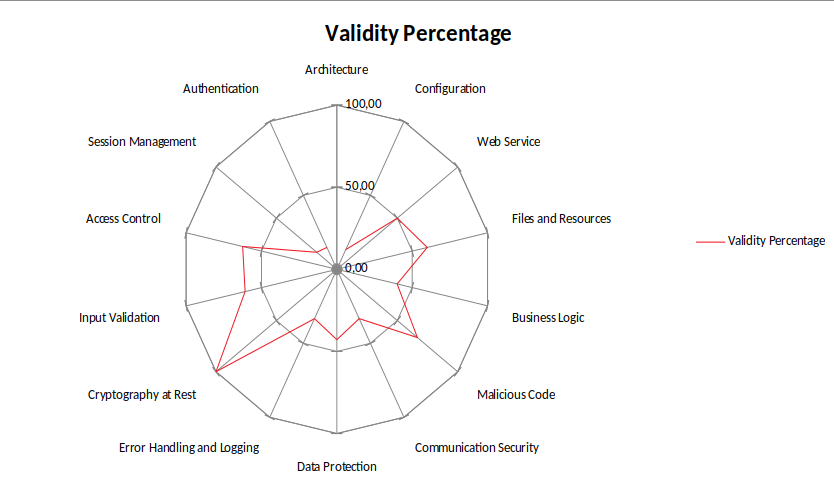
\includegraphics[width=16cm]{images/ASVS Results.png}
      \caption{Resultado da Auditoria: Validity Percentage}
      \label{fig:asvs_valid}
\end{figure}

\begin{figure}[H]
      \centering
      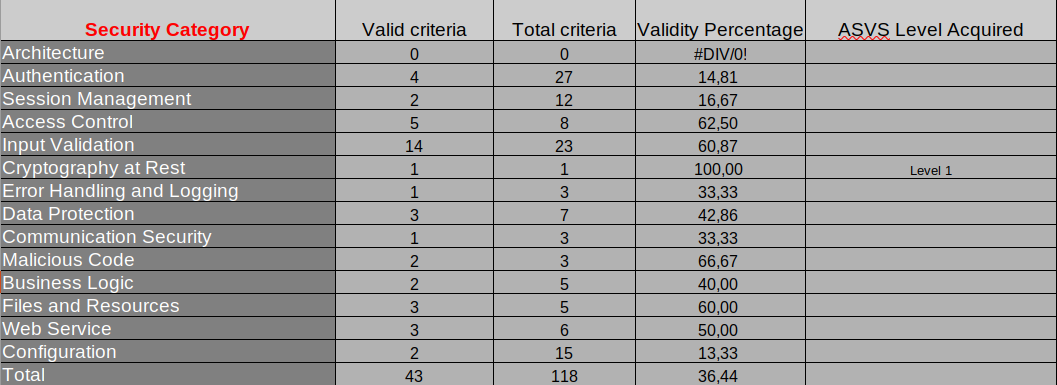
\includegraphics[width=16cm]{images/ASVS Results Tab.png}
      \caption{Resultado da Auditoria: Results Tabel}
      \label{fig:asvs_tab}
\end{figure}

Como se pode analisar pelas imagens anteriores, o projecto original (presente na pasta \textbf{\textit{app\_org}} contém diversos problemas de segurança e na sua correção será dada prioridade às 10 questões mais importantes e urgentes, conforme definido pelo \textit{OWASP Top Ten}. Também serão corrigidas as  vulnerabilidades consideradas importantes pelos elementos responsáveis do grupo do projeto. No auxílio a essas correções serão implementadas duas novas funcionalidades (referidas em \ref{chap.Intro}):

\begin{enumerate}
    \item \textbf{\textit{Multi-factor Authentication (\ac{mfa})}}
    \item \textbf{\textit{Password Strength Evaluation}}
\end{enumerate}

\section{Selecção de Vulnerabilidades}

Após análise dos resultados demonstrados em reunião geral com os elementos do grupo do projeto, foram selecionadas diversas vulnerabilidades que exigem uma correção prioritária, visto que constituem uma maior ameaça:


\textbf{Nota:}\textit{o simbolo * indica que vulnerabilidades (problema) está correlacionado de certa forma.}

\begin{itemize}
    \item 4.0.2-2.1.5 
    \item 4.0.2-5.2.5 *
    \item 4.0.2-5.2.8 *
    \item 4.0.2-5.5.1 *
    \item 4.0.2-8.2.1
    \item 4.0.2-8.3.4
    \item 4.0.2-12.1.1
    \item 4.0.2-13.2.2
    \item 4.0.2-14.2.2
    \item 4.0.2-14.3.2 *
    \item 4.0.2-14.4.3  
\end{itemize}

Para além das vulnerabilidades que exigem uma correção prioritária, foram selecionadas algumas vulnerabilidades extra que irão também contribuir para a mitigação dos problemas de segurança detetados. \textit{"secundária"}:

\begin{itemize}
    \item 4.0.2-2.1.1
    \item 4.0.2-2.1.2
    \item 4.0.2-2.1.7
    \item 4.0.2-2.1.8
    \item 4.0.2-2.1.12
    \item 4.0.2-3.2.3 *
    \item 4.0.2-3.3.1 *
    \item 4.0.2-3.4.1
    \item 4.0.2-3.4.2
    \item 4.0.2-3.4.3
    \item 4.0.2-3.4.4
    \item 4.0.2-5.1.5
    \item 4.0.2-8.3.3
    \item 4.0.2-14.3.3
    \item 4.0.2-14.4.2
    \item 4.0.2-14.4.5
    \item 4.0.2-14.4.6
\end{itemize}

%
%%%%%%%%%%%%%%%%%%%%%%%%%%%%%%%%%%%%%%%%%%%%%%%%%%%%%%%%%
%%%%%CAPÍTULO 3: LISTA DE VULNERABILIDADES E CORRECÇÕES
%
\chapter{Correcção: Mitigação de Vulnerabilidades Detectadas}
\label{chap.Correcao}
\pagenumbering{arabic}


\section{Correcções Prioritárias:}

%%%%%%%%%%%%%%%%%%%%%%%%%%%%%%%%%%%%%%
%%%%%%%%%%%%%%%%%%%%%%%%%%%%%%%%%%%%%%
\subsection*{Requisito: 4.0.2-2.1.5}
O 5º requisito \ac{asvs} do capítulo 2 (\textit{"Authentication"}), secção 1  (\textit{"Password Security Credentials"}) foi detetado através da análise manual do código.
Na deteção foram identificadas falhas no sistema de alteração de passwords para utilizadores verificados. Estas falhas não permitiam a realização desta ação e foram corrigidas.  

%%%%%%%%%%%%%%%%%%%%%%%%%%%%%%%%%%%%%%
%%%%%%%%%%%%%%%%%%%%%%%%%%%%%%%%%%%%%%
\subsection*{Requisito: 4.0.2-5.2.5}

O 5º requisito \ac{asvs} do capítulo 5 (\textit{"Input Validation"}), secção 2  (\textit{"Sanitization and Sandboxing Requirements"}) foi detectado através da ferramenta automática, Bandit (Python), no ficheiro \textbf{app\_sec.py}, como se pode visualizar na Figura \ref{fig:det5.2.5}:

\begin{figure}[H]
      \centering
      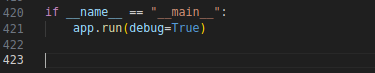
\includegraphics[width=10cm]{images/detdebug.png}
      \caption{Detecção Bandit - Requisito: 4.0.2-5.2.5 - (app\_sec.py)}
      \label{fig:det5.2.5}
\end{figure}

De forma a proteger ainda mais a aplicação contra \textit{"template injection attacks"} e por forma a solucionar a CWE-94, \textit{"CWE-94: Improper Control of Generation of Code ('Code Injection')"}, foi efectuada a seguinte correcção de código Backend (Figura \ref{fig:cor5.2.5}):

\begin{figure}[H]
      \centering
      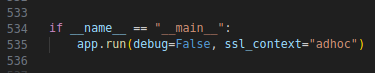
\includegraphics[width=10cm]{images/cordebug.png}
      \caption{Correcção Bandit - Requisito: 4.0.2-5.2.5 - (app\_sec.py)}
      \label{fig:cor5.2.5}
\end{figure}

Neste caso, debug deve estar desactivado para evitar injecção de código arbitrário de um potencial atacante.

%%%%%%%%%%%%%%%%%%%%%%%%%%%%%%%%%%%%%%
%%%%%%%%%%%%%%%%%%%%%%%%%%%%%%%%%%%%%%
\subsection*{Requisito: 4.0.2-5.2.8}

O 8º requisito \ac{asvs} do capítulo 5 (\textit{"Input Validation"}), secção 2  (\textit{"Sanitization and Sandboxing Requirements"}) foi detectado através da ferramenta automática, Bandit (Python), no ficheiro \textbf{app\_sec.py}.

\begin{figure}[H]
      \centering
      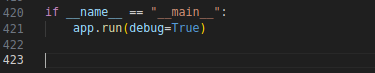
\includegraphics[width=10cm]{images/detdebug.png}
      \caption{Detecção Bandit - Requisito: 4.0.2-5.2.5 - (app\_sec.py)}
      \label{fig:det5.2.8}
\end{figure}

De forma a proteger ainda mais a aplicação contra por forma a que os conteúdos fornecidos aos utilizadores seja restringidos (ou desactivados), e por forma a solucionar a CWE-94, \textit{"CWE-94: Improper Control of Generation of Code ('Code Injection')"}, foi efectuada a seguinte correcção de código Backend (Figura \ref{fig:cor5.2.8}):

\begin{figure}[H]
      \centering
      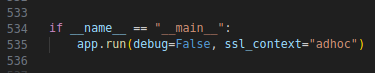
\includegraphics[width=10cm]{images/cordebug.png}
      \caption{Correcção Bandit - Requisito: 4.0.2-5.2.5 - (app\_sec.py)}
      \label{fig:cor5.2.8}
\end{figure}

Neste caso, debug deve estar desactivado para evitar injecção de código arbitrário de um potencial atacante.

%%%%%%%%%%%%%%%%%%%%%%%%%%%%%%%%%%%%%%
%%%%%%%%%%%%%%%%%%%%%%%%%%%%%%%%%%%%%%
\subsection*{Requisito: 4.0.2-5.5.1}

O 8º requisito \ac{asvs} do capítulo 5 (\textit{"Input Validation"}), secção 2  (\textit{"Sanitization and Sandboxing Requirements"}) foi detectado através da análise manual do código Backend presente no ficheiro \textbf{app\_sec.py}:

\begin{figure}[H]
      \centering
      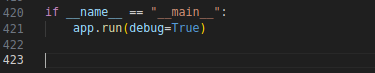
\includegraphics[width=10cm]{images/detdebug.png}
      \caption{Detecção Bandit - Requisito: 4.0.2-5.2.5 - (app\_sec.py)}
      \label{fig:det5.5.1}
\end{figure}

Neste, por uma questão de segurança, deve ser ativado HTTPS com SSL, tal como demonstrado na Figura \ref{fig:cor5.5.1}:

\begin{figure}[H]
      \centering
      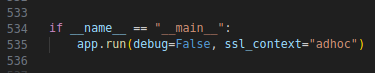
\includegraphics[width=10cm]{images/cordebug.png}
      \caption{Correcção Bandit - Requisito: 4.0.2-5.2.5 - (app\_sec.py)}
      \label{fig:cor5.5.1}
\end{figure}

No entanto, esta alteração gera um certificado auto-assinado para fins de desenvolvimento, pelo que é importante no \textit{deployment} alterar por forma a conter um certificado de uma Autoridade Certificadora (CA) de confiança, permitindo assim que seja reconhecido pelo browsers modernos mantendo confiança e segurança. 

%%%%%%%%%%%%%%%%%%%%%%%%%%%%%%%%%%%%%%
%%%%%%%%%%%%%%%%%%%%%%%%%%%%%%%%%%%%%%
\subsection*{Requisito: 4.0.2-8.2.1}
O 1º requisito \ac{asvs} do capítulo 8 (\textit{"Data Protection"}), secção 2 (\textit{"Client-side Data Protection"}), foi detectado através da análise manual do código Backend presente no ficheiro \textbf{app\_sec.py}. Neste, não são definidos cabeçalhos \textit{"anti-caching"} por forma a evitar que dados sensíveis sejam armazenados em cache nos browsers modernos, como se pode verificar na Figura \ref{fig:det8.2.1}:

\begin{figure}[H]
      \centering
      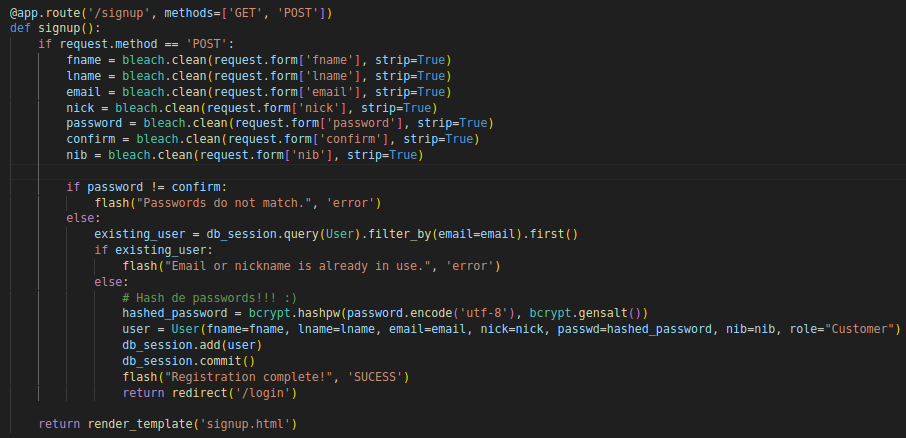
\includegraphics[width=16cm]{images/Detecção_8_2_1.png}
      \caption{Exemplo de Detecção - Requisito: 4.0.2-8.2.1 - (app\_sec.py, rota signup )}
      \label{fig:det8.2.1}
\end{figure}


Assim, por forma a corrigir este problema, foram implementadas respostas (responses) encapsuladas em cabeçalhos com instruções de controlo de cache, como podemos analisar na Figura \ref{fig:cor8.2.1}:


\begin{figure}[H]
      \centering
      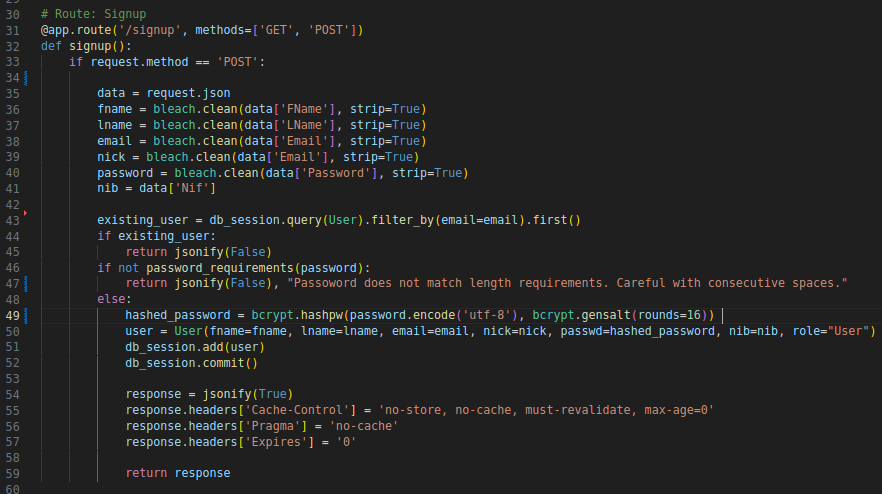
\includegraphics[width=16cm]{images/Correcção_8_2_1.png}
      \caption{Correcção - Requisito: 4.0.2-8.2.1 - (app\_sec.py, rota \_signup )}
      \label{fig:cor8.2.1}
\end{figure}

A principal alteração foi a adição de cabeçalhos de controlo de cache (Cache-Control, Pragma e Expires) na resposta (response) encapsulada nestes. que indicam explicitamente que o conteúdo não deve ser armazenado, evitando assim persistência de dados sensíveis em caches não controladas de browsers, anulando a possibilidade das informações sejam "recuperadas" por utilizadores não autorizados (atacantes).

%%%%%%%%%%%%%%%%%%%%%%%%%%%%%%%%%%%%%%
%%%%%%%%%%%%%%%%%%%%%%%%%%%%%%%%%%%%%%
\subsection*{Requisito: 4.0.2-8.3.4}

O 8º requisito \ac{asvs} do capítulo 14 (\textit{"Data Protection"}), secção 3  (\textit{"Sensitive Private Data"}) foi detectado através da ferramenta automática OWASP ZAP, no ficheiro \textbf{app\_inserts.py}.
O não cumprimento deste requisito pode resultar na exposição de dados sensíveis.


Para resolver essa questão, foram eliminados todos os comentários e possíveis mensagem de erro que poderiam guiar utilizadores maliciosos a descobrir vulnerabiliades no website e aplicação.

É importante destacar que uma política de processamento de dados sensíveis já estava em vigor na versão anterior do projeto. Essa política consistia na aplicação de técnicas de criptografia para proteger os dados sensíveis durante o armazenamento, garantindo uma camada adicional de segurança.

%%%%%%%%%%%%%%%%%%%%%%%%%%%%%%%%%%%%%%
%%%%%%%%%%%%%%%%%%%%%%%%%%%%%%%%%%%%%%
\subsection*{Requisito: 4.0.2-12.1.1}

O 1º requisito \ac{asvs} do capítulo 12 (\textit{"Files and Resources"}), secção 1 (\textit{"File Upload Requirements"}, foi detectado através da ferramente automática Snyk.

Esta vulnerabilidade afeta um pacote utilizado (@adobe/css-tools) afectando selectors de CSS inválidos e manipulando os mesmos. Ao aceitar ficheiros de grande dimensão, estes podem provocar uma exposição a ataques de Negação de Serviço (REDoS/DoS) ao website.

Para corrigir esta vulnerabilidade foram atualizadas as bibliotecas testing-library/jest-dom e  adobe/css-tools, utilizadas no frontend, para as versões 5.17.0 e 4.3.2, respetivamente.

%%%%%%%%%%%%%%%%%%%%%%%%%%%%%%%%%%%%%%
%%%%%%%%%%%%%%%%%%%%%%%%%%%%%%%%%%%%%%
\subsection*{Requisito: 4.0.2-13.2.2}

O 2º requisito \ac{asvs} do capítulo 13 (\textit{"Web Services"}), secção 2  (\textit{"RESTful Web Service Verification Requirements"}) foi detectado através da ferramente automática Snyk.


Esta vulnerabilidade foi corrigida pela atualização da biblioteca \textit{"postcss"} para uma versão superior ou igual a 8.4.31, permitindo que os dados transmitidos em JSON estivessem no formato correto.


%%%%%%%%%%%%%%%%%%%%%%%%%%%%%%%%%%%%%%
%%%%%%%%%%%%%%%%%%%%%%%%%%%%%%%%%%%%%%
\subsection*{Requisito: 4.0.2-14.2.2}

O 2º requisito \ac{asvs} do capítulo 14 (\textit{"Configuration"}), secção 2  (\textit{"Dependency"}) foi detectado através através da análise manual do código.
O não cumprimento deste requisito pode levar a falhas de segurança.

Para resolver essa questão, todos os utilizadores de teste e administradores foram removidos no processo de criação da base de dados. Essa medida visa garantir que informações sensíveis não estejam presentes em ambientes de produção.

A remoção dos administradores, em espefíco, do código também contribuiu para reforçar a segurança, uma vez que a presença de contas de administrador poderia representar um risco significativo. Se tais contas permanececem no ficheiro \textbf{ db\_inserts}, podiam ser exploradas por atacantes que tentam obter privilégios não autorizados. Além disso, a existência de administradores não necessários aumenta o risco de ataques e pode resultar em ações não autorizadas que requerem privilégios elevados.


%%%%%%%%%%%%%%%%%%%%%%%%%%%%%%%%%%%%%%
%%%%%%%%%%%%%%%%%%%%%%%%%%%%%%%%%%%%%%
\subsection*{Requisito: 4.0.2-14.3.2}

O 2º requisito \ac{asvs} do capítulo 14 (\textit{"Configuration"}), secção 3  (\textit{"Unintended Security Disclosure Requirements"}) foi detectado através da análise manual do código, no ficheiro \textbf{app\_sec.py}.
O não cumprimento deste requisito pode resultar na exposição de dados sensíveis dos utilizadores, assim como vulnerabilidades presentes no website e na aplicação, devido à possível divulgação de mensagens de erro."


Para corrigir este problema, quando se pretende executar a aplicação Flask modo de debug enconta-se desativado, ou seja, com a opção definida como False.

\begin{figure}[H]
      \centering
      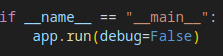
\includegraphics[width=8cm]{images/14_3_2.png}
      \caption{Correção do Requisito: 4.0.2-14.3.2 - (app\_sec.py)}
      \label{fig:det14_3_2}
\end{figure}


%%%%%%%%%%%%%%%%%%%%%%%%%%%%%%%%%%%%%%
%%%%%%%%%%%%%%%%%%%%%%%%%%%%%%%%%%%%%%
\subsection*{Requisito: 4.0.2-14.4.3}
O 3º requisito \ac{asvs} do capítulo 14 (\textit{"Configuration"}), secção 4  (\textit{"HTTP Security Headers Requirements"}) foi detectado através da ferramenta automática OWASP ZAP.
O não cumprimento deste requisito deixa o website mais vulnerável a ameaças, como ataques JavaScript injection, Cross-Site Scripting, entre outros.

Para mitigar esta vulnerabilidade foram adicionados cabeçalho CSP a todas às respostas HTTP feitas pelo backend. Os cabeçalhos adicionados têm como por objetivo evitar problemas de segurança relacionados ao armazenamento em cache, garantido assim, que as respostas não serão armazenadas localmente nos dispositivos dos utilizadores.

A figura \ref{fig:exemplo14_4_3} é um exemplo de um cabeçalho adicionado a uma resposta de modo a obter a segurança pretendida.


\begin{figure}[H]
      \centering
      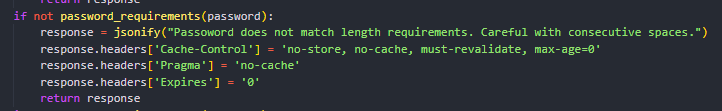
\includegraphics[width=14cm]{images/exemplo14_4_3.png}
      \caption{Exemplo da correção do requisito: 4.0.2-14.4.3 - (app\_sec.py)}
      \label{fig:exemplo14_4_3}
\end{figure}




%%%%%%%%%%%%%%%%%%%%%%%%%%%%%%%%%%%%%%%%%%%%%%%%%%%%%%%%%%%%%%%%%%%%%%%%%%%%%%%%%%%%%%%%%%%%%%%%%%%%%%%%%
\section{Correcções Secundárias:}


\subsection*{Requisito: 4.0.2-2.1.1 e 4.0.2-2.1.2}
O 1º e 2º requisito \ac{asvs} do capítulo 2 (\textit{"Authentication"}), secção 1  (\textit{"Password Security Credentials"}) foi detetado através da análise manual do código.

Para corrigir esta vulnerabilidade, no backend foi criada uma função que garanta que as passwords cumpram um conjunto de  requesitos. Esses requesitos são:

\begin{enumerate}
    \item Passwords têm obrigatoriamente de ter um tamanho superior a 12 caracteres. Múltiplos espaços consecutivos são contados como apenas um carácter
    \item Passwords não podem ter um tamanho superior a 128 caracteres.
\end{enumerate}

Aqui podemos ver como estes requesitos são verificados.

\begin{figure}[H]
      \centering
      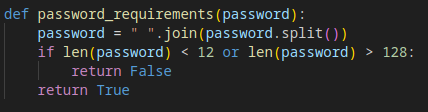
\includegraphics[width=14cm]{images/pass_req.png}
      \caption{Correcção - Requisito: 4.0.2-2.1.1 e 2.1.2 - (app\_sec.py)}
      \label{fig:pass_req}
\end{figure}

Aqui podemos ver como a função é utilizada.

\begin{figure}[H]
      \centering
      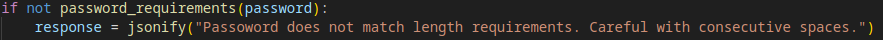
\includegraphics[width=14cm]{images/use_pass_req.png}
      \caption{Correcção - Requisito: 4.0.2-2.1.1 e 2.1.2 - (app\_sec.py)}
      \label{fig:use pass_req}
\end{figure}


%%%%%%%%%%%%%%%%%%%%%%%%%%%%%%%%%%%%%%
%%%%%%%%%%%%%%%%%%%%%%%%%%%%%%%%%%%%%%
\subsection*{Requisito: 4.0.2-2.1.7}
O 7º requisito \ac{asvs} do capítulo 2 (\textit{"Authentication"}), secção 1  (\textit{"Password Security Credentials"}) foi detetado através da análise manual do código.

Esta vulnerabilidade foi corrigida aplicando a função \texttt{lookup\_pwned\_api\_password} no backend que retorna se a password foi encontrada em data breaches ou não. Caso tenha sido, um popup irá alertar o utilizador desta vulnerabilidade e encaminhá-lo para a página de alteração de password.
\begin{figure}[H]
      \centering
      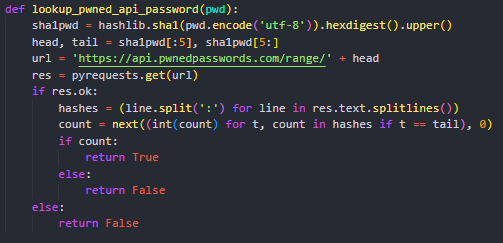
\includegraphics[width=14cm]{images/lookup_pwned_api_password.png}
      \caption{Correcção - Requisito: 4.0.2-2.1.7  - (app\_sec.py)}
      \label{fig:lookup_pwned_api_password}
\end{figure}


%%%%%%%%%%%%%%%%%%%%%%%%%%%%%%%%%%%%%%
%%%%%%%%%%%%%%%%%%%%%%%%%%%%%%%%%%%%%%
\subsection*{Requisito: 4.0.2-2.1.8}
O 8º requisito \ac{asvs} do capítulo 2 (\textit{"Authentication"}), secção 1  (\textit{"Password Security Credentials"}) foi detetado através da análise manual do código.

\begin{figure}[H]
      \centering
      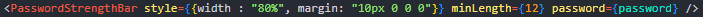
\includegraphics[width=16cm]{images/2_1_8.png}
      \caption{Correcção - Requisito: 4.0.2-2.1.8  - (RegisterPage.js)}
      \label{fig:2_1_8}
\end{figure}

A correção desta vulnerabilidade baseou-se na adição de uma barra indicadora, que demonstra de forma visual e intuitiva a força da password que o utilizador deseja utilizar. O resultado desta implementação pode ser verificado pela figura \ref{fig:2_1_8_barra}.
\begin{figure}[H]
      \centering
      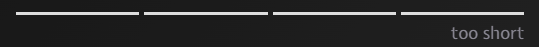
\includegraphics[width=16cm]{images/2_1_8_barra.png}
      \caption{Correcção - Requisito: 4.0.2-2.1.8  - (RegisterPage.js)}
      \label{fig:2_1_8_barra}
\end{figure}

%%%%%%%%%%%%%%%%%%%%%%%%%%%%%%%%%%%%%%
%%%%%%%%%%%%%%%%%%%%%%%%%%%%%%%%%%%%%%
\subsection*{Requisito: 4.0.2-2.1.12}
O 12º requisito \ac{asvs} do capítulo 2 (\textit{"Authentication"}), secção 1  (\textit{"Password Security Credentials"}) foi detetado através da análise manual do código.

Esta vulnerabilidade apenas ocorria na página de alteração de password. Portanto, foi mitigada nesta página pela aplicação de mecanismos anteriormente aplicados noutras páginas que envolvem passwords.

%%%%%%%%%%%%%%%%%%%%%%%%%%%%%%%%%%%%%%
%%%%%%%%%%%%%%%%%%%%%%%%%%%%%%%%%%%%%%
\subsection*{Requisito: 4.0.2-3.4.1}

O 3º requisito \ac{asvs} do capítulo 3 (\textit{"Session\_Management"}), secção 4  (\textit{"Cookie-based Session Management"}) foi detetado através da análise manual do código.

Esta vulnerabilidade apenas ocorria na criação do cookie de sessão. Portanto, foi corrigida fornecendo ao cookie de sessão o parametro necessário para obter o paramtro fornecido.

%%%%%%%%%%%%%%%%%%%%%%%%%%%%%%%%%%%%%%
%%%%%%%%%%%%%%%%%%%%%%%%%%%%%%%%%%%%%%
\subsection*{Requisito: 4.0.2-3.4.2}

O 3º requisito \ac{asvs} do capítulo 3 (\textit{"Session\_Management"}), secção 4  (\textit{"Cookie-based Session Management"}) foi detetado através da análise manual do código.

Esta vulnerabilidade apenas ocorria na criação do cookie de sessão. Portanto, foi corrigida fornecendo ao cookie de sessão o parametro necessário para obter o paramtro fornecido.

%%%%%%%%%%%%%%%%%%%%%%%%%%%%%%%%%%%%%%
%%%%%%%%%%%%%%%%%%%%%%%%%%%%%%%%%%%%%%
\subsection*{Requisito: 4.0.2-3.4.3}

O 3º requisito \ac{asvs} do capítulo 3 (\textit{"Session\_Management"}), secção 4  (\textit{"Cookie-based Session Management"}) foi detetado através da análise manual do código.

Esta vulnerabilidade apenas ocorria na criação do cookie de sessão. Portanto, foi corrigida fornecendo ao cookie de sessão o parametro necessário para obter o paramtro fornecido.

%%%%%%%%%%%%%%%%%%%%%%%%%%%%%%%%%%%%%%
%%%%%%%%%%%%%%%%%%%%%%%%%%%%%%%%%%%%%%
\subsection*{Requisito: 4.0.2-8.3.3}

O 3º requisito \ac{asvs} do capítulo 8 (\textit{"Data Protection"}), secção 1  (\textit{"Sensitive Private Data"}) foi detetado através da análise manual do código.
O não cumprimento deste requisito pode resultar em uma quebra de confiança entre o website e os clientes, pois estes não têm uma compreensão clara de como seus dados sensíveis podem ser utilizados.

Para lidar com esse problema, foram implementados\textit{ "Termos e Condições"}. Todos os utiliadores são obrigados a aceitar ou rejeitar esses termos. Dependendo da resposta do utilizador, o acesso ao website ou a outras funcionalidades pode ser concedido ou negado.

\begin{figure}[H]
      \centering
      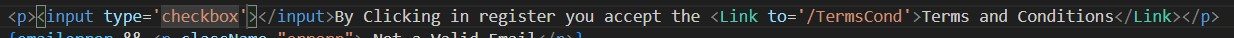
\includegraphics[width=14cm]{images/T&C.jpg}
      \caption{Correcção - Requisito: 4.0.2-8.3.3}
      \label{fig:T&C}
\end{figure}

Ao criar \textit{"Termos e Condições"} promovemos transparência com os utilizadores, uma vez que eles têm conhecimento de como os seus dados podem ser usados. Essa abordagem reflete um compromisso com a comunicação clara e a proteção da privacidade dos utilizadores.




%%%%%%%%%%%%%%%%%%%%%%%%%%%%%%%%%%%%%%%%%%%%%%%%%%%%%%%%%
%%%%%CAPÍTULO 4: MULTI-FACTOR AUTHENTICATION (MFA)
%

\chapter{Software Features}
Foram implementadas duas funcionalidades de software com o objetivo de melhorar a segurança do website. As funcionalidades escolhidas para implementar foram:

\begin{itemize}
\item Password Strength Evaluation
\item \ac{mfa} com OAuth2.0 e Google Identity
\end{itemize}

\section{Password Strength Evaluation}

A necessidade de passwords fortes e seguras é essencial para a segurança do website e do utilizador.
Para cumprir este requisito, foram aplicadas medidas imperativas para a criação ou alteração de uma password, tais como, a verificação de tamanho e variedade de caracteres usados, a avaliação da força da password e a verificação de correspondências com data breaches. 

Para garantir uma password forte, na sua criação ou alteração é verificado se cumpre os critérios impostos. Esta operação pode-se observar pela figura \ref{fig:2_1_1e2-feature}.
\begin{figure}[H]
      \centering
      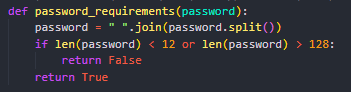
\includegraphics[width=10cm]{images/2_1_1e2.png}
      \caption{Função de verificação da password  - (app\_sec.py)}
      \label{fig:2_1_1e2-feature}
\end{figure}

Finalmente, para a verificação de correspondências com data breaches, a função \texttt{lookup\_pwned\_api\_password} foi implementada, fazendo uso da API do Have I Been Pwned. Esta função verifica se a password já foi descoberta em data breaches e consequentemente insegura.
Também foi verificado que esta api é segura devido ao uso da propriedade k-anonymity, onde apenas é fornecido os primeiros 5 caracteres do hash da password para a api retornar uma lista de hashes de passwords. A partir dessa lista é procurado o hash completo igual ao hash da password a ser avaliada para então tirar conclusões. Esta função pode ser analisada pela figura\ref{fig:lookup_pwned_api_password-feature}.
\begin{figure}[H]
      \centering
      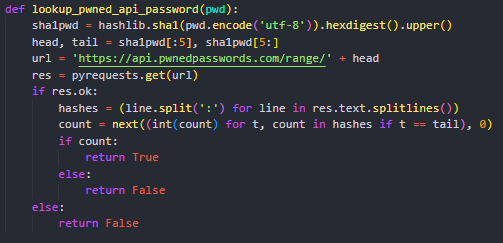
\includegraphics[width=14cm]{images/lookup_pwned_api_password.png}
      \caption{Função lookup\_pwned\_api\_password  - (app\_sec.py)}
      \label{fig:lookup_pwned_api_password-feature}
\end{figure}

\section{\ac{mfa}}

A autenticação de múltiplos fatores (\ac{mfa}) é uma medida crucial para reforçar a segurança do acesso ao website, por parte de utilizadores. Optámos por implementar o OAuth2.0 com o Google Identity.

Google Identity é um serviço de gestão de identidade fornecido pelo Google. Permite que os utilizadores se autentiquem em diversas aplicações e serviços usando as suas credenciais do Google. Ao integrar o Google Identity no nosso website, beneficiamos da segurança robusta proporcionada pelo Google, incluindo verificações de autenticação em dois fatores e deteção de atividades suspeitas.

O OAuth2.0 é um protcolo de autorizção utilizado por aplicações de modo a permitir que aplicações obtenham acesso a recursos em nome de utilizadores sem relevaram as suas credencias.

O processo de autenticação com \ac{mfa}, usando o Google Identity e OAuth 2.0, segue os seguintes passos:

\begin{enumerate}
\item O utilizador seleciona a opção de login com Google no nosso website.
\item O website redireciona o utilizador para o serviço de autenticação do Google usando OAuth 2.0.
\item O utilizador introduz as suas credenciais da sua conta do Google.
\item Após a autenticação bem-sucedida da conta do utilizador, o Google Identity gera um \ac{jwt} Token de acesso.
\item O frontend envia o \ac{jwt} Token para o backend. 
\item O backend verifica o token de acesso com o Google Identity para garantir a sua autenticidade. Caso essa autenticidade seja verificada o backend sinaliza o frontend criando assim a sessão do utilizador.
\end{enumerate}

Esta abordagem proporciona uma camada adicional de segurança, garantindo que apenas utilizadores autorizados, que passaram pela autenticação em dois fatores, possam aceder ao website.

Envio do \ac{jwt} Token do frontend para o backend.

 \begin{figure}[H]
      \centering
      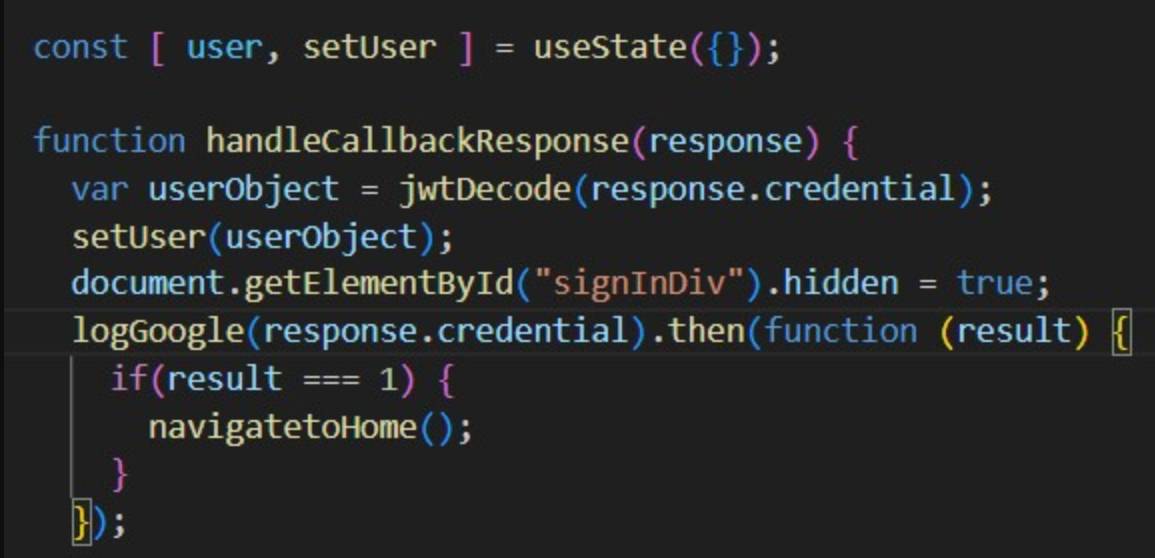
\includegraphics[width=16cm]{images/google_login_front.png}
      \caption{Função responsável pela obtenção do \ac{jwt} Token}
      \label{fig:login_google}
    \end{figure}

 \begin{figure}[H]
      \centering
      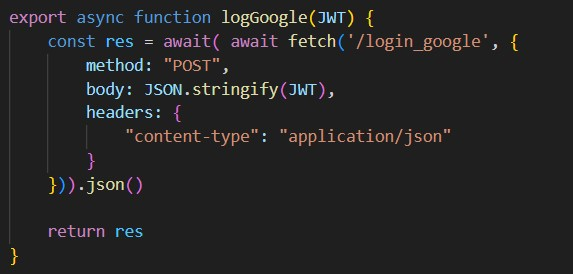
\includegraphics[width=16cm]{images/call_login_google.jpg}
      \caption{Função responsável pelo envio do \ac{jwt} Token para o backend}
      \label{fig:login_google}
    \end{figure}

De modo a verificar a autentencidade da \ac{jwt} Token enviada pelo frontend recorremos à função verify\_google\_token.
Após essa vaidação realizamos o login do utilizador

   \begin{figure}[H]
      \centering
      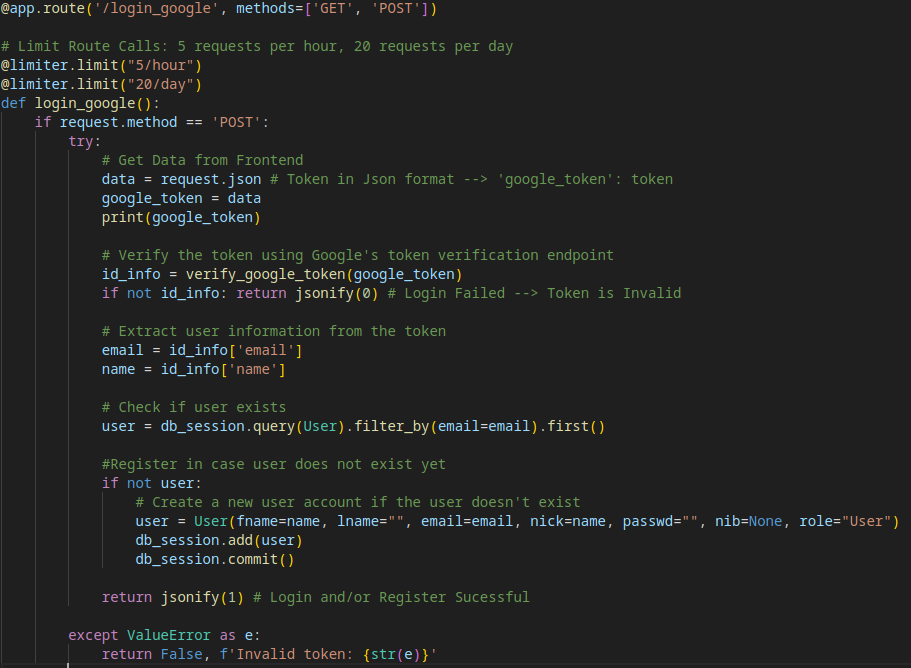
\includegraphics[width=16cm]{images/MFA_login_google.png}
      \caption{Rota responável pela verificação do \ac{jwt} Token e o login do utilizador}
      \label{fig:login_google}
    \end{figure}

Contactamos o Google Token verification endpoint para garantir a autenticidade do Token.

   \begin{figure}[H]
      \centering
      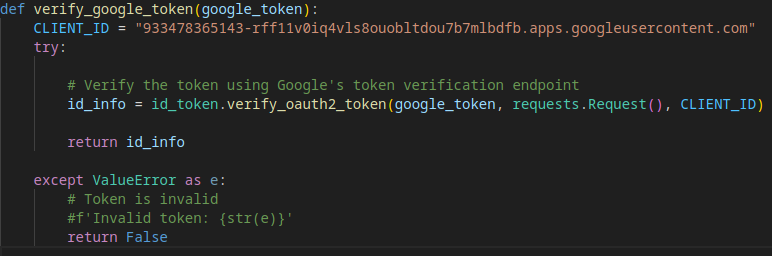
\includegraphics[width=16cm]{images/verify_token.png}
      \caption{Função verify\_google\_token}
      \label{fig:verify_google_token}
    \end{figure}


%%%%%%%%%%%%%%%%%%%%%%%%%%%%%%%%%%%%%%%%%%%%%%%%%%%%%%%%%
%%%%%CONCLUSÃO
%
\chapter*{Conclusão:}
\label{chap.conclusão}
\lhead{Conclusão}

Em conclusão, este projeto desempenhou um papel fundamental na elevação dos padrões de segurança da loja online de memorabilia do \ac{deti}. A auditoria de segurança de nível 1, baseada no \ac{asvs} proporcionou uma visão abrangente das vulnerabilidades presentes na aplicação, possibilitando a implementação de correções das mesmas.

A identificação e resolução das principais questões de segurança, delineadas pelo \ac{asvs}, não fortaleceram apenas a resistência da aplicação a potenciais ameaças, mas também contribuíram para a melhoria geral da integridade e confidencialidade dos dados dos utilizadores. A explicação detalhada do impacto das correções evidencia o compromisso com a construção de uma aplicação robusta e a sua segurança.

Além da correção das vulnerabiliades detetadas, provenientes da realização da auditoria, a adição de duas novas funcionalidades, Autenticação Multi-Fator (\ac{mfa}) com OAuth 2.0 e Google Identity, juntamente com a avaliação da força de senha por meio de um serviço externo, aumentou significativamente a segurança da loja online, Detitalismo.

Este projecto ilustra claramente as consequências significativas no mundo real das práticas seguras de programação para aplicações e/ou soluções Web. A negligência em relação às boas práticas e segurança pode resultar em violações de dados e privacidade, perdas financeiras, furto de identidade e danos à reputação de uma organização ou utilizador comum.

Contudo, é fundamental referir que, apesar de todo o esforço e empenho disponibilizado neste projecto, ainda existem vulnerabilidades presentes, as quais podem ser usadas por um potencial atacante. Esta situação deve-se ao facto de, na opinião dos elementos dos grupo de trabalho, serem necessárias posteriores auditorias para corrigir todos os erros e vulnerabilidades presentes.

Assim, o grupo de trabalho gostaria de reforçar a ideia de que auditorias periódicas e uma constante vigilância são fundamentais para proporcionar aplicações web mais seguras e robustas contra ataques maliciosos, protegendo utilizadores e dados tendo em conta Confidencialidade, Integridade e Disponibilidade de serviços.

%
%%%%%%%%%%%%%%%%%%%%%%%%%%%%%%%%%%%%%%%%%%%%%%%%%%%%%%%%%
%%%%%CONTRIBUIÇÕES DE AUTORES:
% 
\chapter*{Contribuições dos Autores}

        Os autores responsáveis pela pesquisa e desenvolvimento do presente projecto, contribuiram de forma coletiva, refletindo-se diversidade de experiências, opiniões e competências que enriqueceram a abordagem ao mesmo. Este projecto pode ser visualizado na sua totalidade na página: \textbf{\url{https://github.com/detiuaveiro/2nd-project-group_26}}. \\

        \textbf{Autores:}
        \begin{itemize}
            \item João Pedro Nunes Vieira, NºMec.: 50458
            \item José Miguel Guardado Silva, Nº Mec.: 103248
            \item Henrique Miguel Escudeiro Cruz, Nº Mec.: 103442
            \item Luís Manuel Trindade Diogo, Nº Mec.: 108668

        \begin{table}[H]
            \centering
            \caption{Contribuições dos Autores.}
            \small
            \begin{tabular}{|c|c|c|c|c|}\hline
                Contribuição & João Vieira & José Silva & Henrique Cruz & Luís Diogo  \\ 
                \hline
        	    Produção de Relatório (LaTex)                           & 25~\% & 25~\% & 25~\% & 25~\% \\
			    Correcções de Projecto iniciais           				& 50~\% & 50~\% & 0~\% & 0~\% \\                
                Identificação ASVS, Testes e Auditoria    				& 80~\% & 0~\% & 20~\% & 0~\% \\
                Correcção de Vulnerabilidades           				& 25~\% & 25~\% & 25~\% & 25~\% \\
                Implementação de 2 Novas Funcionalidades          	    & 0~\% & 10~\% & 40~\% & 40~\% \\  
            \hline
            \end{tabular}
            \label{tab.contribuições}
        \end{table}	
        
        
        \end{itemize}

%
%%%%%%%%%%%%%%%%%%%%%%%%%%%%%%%%%%%%%%%%%%%%%%%%%%%%%%%%%
%%%%%BIBLIOGRAFIA:
%
\begin{thebibliography}{9}

\bibitem{thinkpython} 
Allen Downey
\textit{Think Python - How to Think Like a Computer Scientist}. |
Green Tea Press, 2nd Edition, Version 2.4.0, 2015

\bibitem{segredes} 
André Zúquete
\textit{Segurança em Redes Informáticas}. |
FCA - Editora de Informática LDA, 5th Edition, 2018

\bibitem{Wikipedia}
Wikipédia: Enciclopédia livre. |
\text{ pt.wikipedia.org, acedido 04/12/2023.}

\bibitem{sqlite}
SQLite Website. |
\text{ https://www.sqlite.org/docs.html, acedido 09/12/2021.}

\bibitem{sqlalchemy}
SQLAlchemy Website. |
\text{ https://docs.sqlalchemy.org/en/20/, acedido 09/12/2021.}

\bibitem{mitre}
MITRE: A Community-Developed List of Software and Hardware Weakness Types. |
\text{ https://cwe.mitre.org/index.html, acedido 04/10/2021.}

\bibitem{mitre}
ASVS Checklist - Compatível com ASVS version 4.0.2
\text{https://github.com/shenril/owasp-asvs-checklist, acedido a 21/12/2023}

\bibitem{mitre}
OWASP: Open Web Application Security Project
\text{https://owasp.org/www-project-application-security-verification-standard/, acedido a 27/12/2023}

\bibitem{mitre}
OWASP: Open Web Application Security Project - TOP 10 
\text{https://owasp.org/www-project-top-ten/, acedido a 27/12/2023}

\bibitem{mitre}
OWASP: Open Web Application Security Project - Zed Attack Proxy. |
\text{https://owasp.org/www-project-devsecops-guideline/latest/01b-Linting-Code, acedido a 28/12/2023}



\end{thebibliography}
\end{document}